%%%%%%%%%%%%%%%%%%%%%%%%%%%%%%%%%%%%%%%%%%%%%%%%%%%%%%%%%%%%%%%%%%%%%%%%
% Plantilla TFG/TFM
% Universidad de Murcia. Facultad de Informática
% Realizado por: José Manuel Requena Plens
% Modificado: Pablo José Rocamora Zamora
% Contacto: pablojoserocamora@gmail.com
%%%%%%%%%%%%%%%%%%%%%%%%%%%%%%%%%%%%%%%%%%%%%%%%%%%%%%%%%%%%%%%%%%%%%%%%


\chapter{Introducción}

El entrenamiento de redes neuronales profundas para el análisis de tomogramas de crio-microscopía
electrónica (\textit{cryo-ET}) exige grandes volúmenes de datos anotados cuya obtención
experimental es inviable a escala. La generación de tomogramas sintéticos —volúmenes simulados
con distribuciones realistas de proteínas, membranas y ruido— es la alternativa más extendida
para producir conjuntos de entrenamiento a bajo coste. La calidad de esos datos sintéticos
depende directamente de cuán eficientemente el software de simulación consigue empaquetar
macromoléculas en el volumen de interés.

% \begin{figure}[h]
%     \centering
%     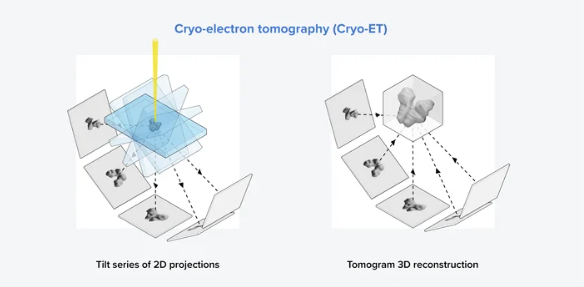
\includegraphics[width=0.80\textwidth]{archivos/cryo-et_schema}
%     \caption{Pipeline de adquisición en cryo-ET: serie de proyecciones 2D a distintos ángulos
%     de inclinación (izquierda) y reconstrucción del tomograma 3D resultante (derecha).}
%     \label{fig:cryo_et_schema}
% \end{figure}

\textit{PolNet}, el marco de simulación de referencia en este ámbito, emplea el algoritmo
\textit{SAWLC} (\textit{Surface Aware Walk from Last Coordinate}) para insertar proteínas en el
volumen. SAWLC produce distribuciones biológicamente plausibles, pero su carácter secuencial y
sus altas tasas de rechazo en volúmenes densos hacen que la generación de un único tomograma
pueda requerir varias horas de CPU, lo que limita severamente la escala de producción de datos.

Este Trabajo Fin de Grado propone \textbf{Tetris~3D}, un algoritmo de inserción de proteínas
basado en correlación cruzada 3D mediante FFT que, en cada paso, identifica globalmente la
posición óptima de colocación en lugar de muestrear candidatos al azar. Se desarrolla además
una versión acelerada por GPU con \textit{CuPy} que reemplaza el bucle de validación de
solapamiento por operaciones vectorizadas completamente en dispositivo, eliminando las
sincronizaciones host-GPU por inserción. El trabajo se articula en un repositorio independiente
cuyo objetivo es comparar Tetris~3D frente a SAWLC y evaluar si constituye un reemplazo viable
para el módulo de inserción de PolNet.

% \begin{figure}[h]
%     \centering
%     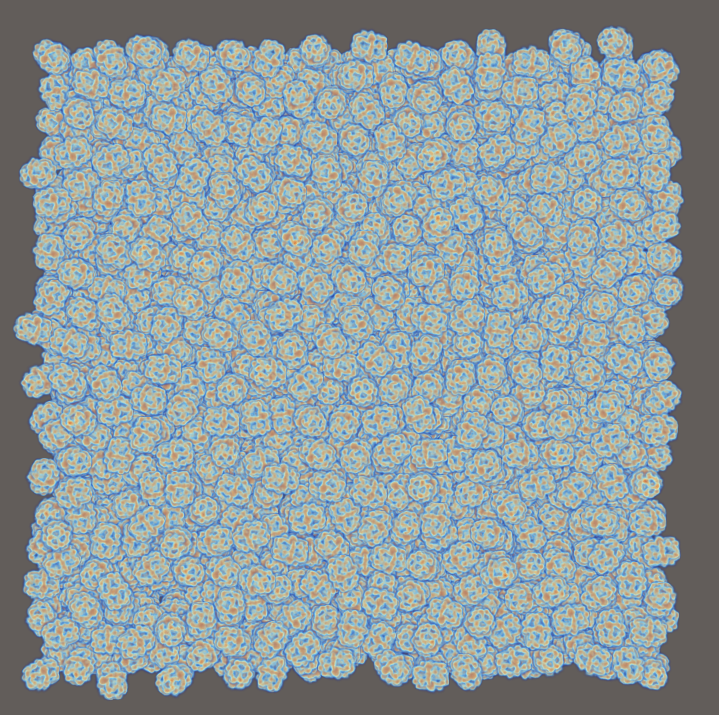
\includegraphics[width=0.55\textwidth]{archivos/tomo_occupany_breakdown}
%     \caption{Vista cenital de un tomograma sintético generado con Tetris~3D, mostrando el
%     denso empaquetamiento volumétrico alcanzado por el algoritmo.}
%     \label{fig:tomo_output}
% \end{figure}

Los objetivos concretos del trabajo son: (i)~implementar el algoritmo Tetris~3D con
correlación FFT 3D para la inserción óptima de macromoléculas; (ii)~desarrollar su versión GPU
minimizando sincronizaciones host-dispositivo mediante la estrategia de doble FFT; (iii)~diseñar
un banco de pruebas que compare ambos algoritmos en ocupancia volumétrica, número de monómeros
insertados y tiempo de ejecución; y (iv)~analizar en qué escenarios Tetris~3D supone una
alternativa competitiva a SAWLC.

El resto del documento se organiza como sigue. El Capítulo~2 revisa el estado del arte:
fundamentos de la adquisición cryo-ET, métodos de generación de datos sintéticos y el
funcionamiento de SAWLC en el contexto de PolNet. El Capítulo~3 recoge el análisis de
requisitos. El Capítulo~4 describe el diseño e implementación de Tetris~3D y del banco de
pruebas. El Capítulo~5 presenta y discute los resultados experimentales. El Capítulo~6 cierra
con las conclusiones y las líneas de trabajo futuro.
